\documentclass[journal]{IEEEtran}

\usepackage{cite}
\usepackage{amsmath,amssymb,amsfonts,amsthm,bm,mathtools}
\usepackage{graphicx}
\usepackage{booktabs,multirow,array}
\usepackage{float}
\usepackage{algorithm}
\usepackage{algpseudocode}
\usepackage{url}
\usepackage{color}
\usepackage{balance}
\usepackage[hidelinks]{hyperref}
\hypersetup{
  pdftitle={Energy-Efficient Hybrid STAR-RIS via Sparse Active Selection and Gain Control},
  pdfauthor={Hongjian Huang, Yunpei Chen, Xingang Xie, Xiaonan Yang, Renjie Liang},
  pdfsubject={Hybrid active-passive STAR-RIS energy efficiency},
  pdfkeywords={STAR-RIS, active RIS, hybrid active-passive RIS, energy efficiency, spectral efficiency, Pareto optimization, amplifier noise}
}
\Urlmuskip=0mu plus 1mu\relax

\graphicspath{{./figs/}{../figs/}}

% Compact IEEE-style float and display spacing.
\setlength{\textfloatsep}{2pt plus 1pt minus 1pt}
\setlength{\floatsep}{2pt plus 1pt minus 1pt}
\setlength{\intextsep}{2pt plus 1pt minus 1pt}
\setlength{\abovedisplayskip}{3pt plus 1pt minus 1pt}
\setlength{\belowdisplayskip}{3pt plus 1pt minus 1pt}
\setlength{\abovedisplayshortskip}{2pt plus 1pt minus 1pt}
\setlength{\belowdisplayshortskip}{2pt plus 1pt minus 1pt}
\setlength{\jot}{1pt}

% Compact section/subsection spacing while preserving IEEEtran heading style.
\makeatletter
\def\section{\@startsection{section}{1}{\z@}{1.2ex plus 0.4ex minus 0.2ex}%
{0.35ex plus 0.2ex minus 0ex}{\normalfont\normalsize\centering\scshape}}%
\def\subsection{\@startsection{subsection}{2}{\z@}{1.05ex plus 0.35ex minus 0.2ex}%
{0.25ex plus 0.15ex minus 0ex}{\normalfont\normalsize\itshape}}%
\makeatother
\setlength{\abovecaptionskip}{1.5pt plus 0.5pt minus 0.5pt}
\setlength{\belowcaptionskip}{0pt}

\let\olditemize\itemize
\let\oldenditemize\enditemize
\renewenvironment{itemize}{\olditemize\setlength{\itemsep}{1pt}\setlength{\parskip}{0pt}\setlength{\parsep}{0pt}}{\oldenditemize}


\newtheorem{proposition}{Proposition}
\DeclareMathOperator{\diag}{diag}
\newcommand{\etaPA}{\eta_{\scriptscriptstyle\mathrm{PA}}}
\newcommand{\mBR}{m_{\scriptscriptstyle\mathrm{BR}}}
\newcommand{\mRU}{m_{\scriptscriptstyle\mathrm{RU}}}

\raggedbottom
\begin{document}

\title{Energy-Efficient Hybrid STAR-RIS via Sparse Active Selection and Gain Control}

\author{Hongjian Huang, Yunpei Chen, Xingang Xie, Xiaonan Yang, and Renjie Liang%
\thanks{Corresponding author: Renjie Liang. Code repository: \url{https://github.com/hjhuang1989-svg/hybrid-star-ris}.}}
\maketitle


\begin{abstract}
Hybrid active-passive simultaneously transmitting and reflecting reconfigurable intelligent surfaces (STAR-RISs) can improve spectral efficiency (SE), but their energy efficiency (EE) is limited by amplifier noise and non-negligible hardware power. This letter studies the energy-splitting (ES) protocol and traces an achievable EE-SE boundary with a multi-component power model that includes base station (BS) power-amplifier power, controller/bias power, switching overhead, and gain-dependent amplification power. The analysis yields an amplification ON-OFF criterion, a closed-form SE-oriented gain law, and an EE-oriented gain refinement, which are integrated with sparse active selection. Simulations under Nakagami-$m$ fading show that sparse active selection reduces BS power at demanding SE targets while avoiding the overhead of a fully active STAR-RIS.
\end{abstract}

\begin{IEEEkeywords}
STAR-RIS, active RIS, hybrid active-passive RIS, energy efficiency, spectral efficiency, Pareto optimization, amplifier noise.
\end{IEEEkeywords}


\section{Introduction}
Reconfigurable intelligent surfaces (RISs) can enhance wireless propagation through passive beam manipulation \cite{wu2019irs,bjornson2020irsrelay,bjornson2020myths}. Simultaneously transmitting and reflecting reconfigurable intelligent surfaces (STAR-RISs) extend this capability to two-side service, allowing one surface to support transmission-side and reflection-side users at the same time \cite{liu2021star,mu2022star}. This two-side operation is attractive for asymmetric coverage, but passive STAR-RIS still suffers from multiplicative path loss, especially when moderate or high spectral efficiency is required.

A direct way to compensate for this loss is to embed active elements into the surface. However, active amplification is not a free array gain: it injects amplifier noise and introduces hardware power consumption \cite{xu2023activestar,ma2023activeee,peng2023hybrid,huang2024hybrid,zhang2022signal}. Measurement-driven RIS studies further show that controller, bias, and switching power should be modeled explicitly rather than absorbed into a single constant \cite{wang2023static,wang2024practical}. These effects are particularly relevant for STAR-RIS because the two sides share aperture, power splitting, and the active-element budget.

Existing active and hybrid RIS/STAR-RIS studies have optimized transmit power, outage, or EE under different hardware assumptions \cite{mu2022star,xu2023activestar,ma2023activeee,peng2023hybrid,huang2024hybrid,zhang2022signal,zhang2023activevspassive}, while measurement-driven studies model controller, unit-cell, and switching-related RIS power separately \cite{wang2023static,wang2024practical}. However, the joint impact of amplifier noise, sparse activation, dynamic switching overhead, and side-wise rate allocation on the EE-SE tradeoff is still not captured under a common ES boundary-generation framework. This motivates an ES-focused design in which the active-noise and hardware-power terms remain explicit in both the gain analysis and the active-selection rule. The contributions are threefold. First, a multi-component EE model is formulated for hybrid active-passive STAR-RIS under ES, separating BS power-amplifier (PA) power, controller/bias consumption, switching overhead, gain-dependent amplification power, and active noise. Second, an analytical gain structure is derived, including an amplification ON-OFF criterion, a closed-form SE-oriented gain law, and an EE-oriented gain refinement for side-wise power minimization. Third, a finite-grid active-set selection and gain-control algorithm is developed to generate achievable EE-SE boundary points under binary activation, side assignment, gain update, and feasibility checking.

\section{System Model}
\subsection{Hybrid Active-Passive STAR-RIS Downlink}
Consider the downlink in Fig.~\ref{fig:system}, where a BS with $M$ antennas serves $K_t$ transmission-side users and $K_r$ reflection-side users through an $N$-element STAR-RIS. The user-index sets are $\mathcal{K}_t=\{1,\ldots,K_t\}$ and $\mathcal{K}_r=\{1,\ldots,K_r\}$. Under the ES protocol \cite{mu2022star}, the $n$th STAR-RIS element is parameterized as
\begin{equation}
\theta_{n,s}=\sqrt{\rho_{n,s}}\beta_{n,s}e^{j\phi_{n,s}},\qquad s\in\{t,r\},
\label{eq:theta}
\end{equation}
where $\rho_{n,s}$ is the power-splitting coefficient, $\beta_{n,s}$ is the amplification factor, and $\phi_{n,s}$ is the phase shift. The coefficients satisfy $\rho_{n,t}+\rho_{n,r}=1$, $0\le \rho_{n,s}\le 1$, and $1\le \beta_{n,s}\le \beta_{\max}$. Passive elements use $\beta_{n,s}=1$, whereas active elements use $\beta_{n,s}>1$ on the side to which they are assigned. Let $\mathcal{A}_t$ and $\mathcal{A}_r$ denote the active-element sets for transmission and reflection. Each active element is assigned to at most one side. Hence $\mathcal{A}_t\cap\mathcal{A}_r=\emptyset$ and $\mathcal{A}=\mathcal{A}_t\cup\mathcal{A}_r$.

\begin{figure}[!t]
\centering
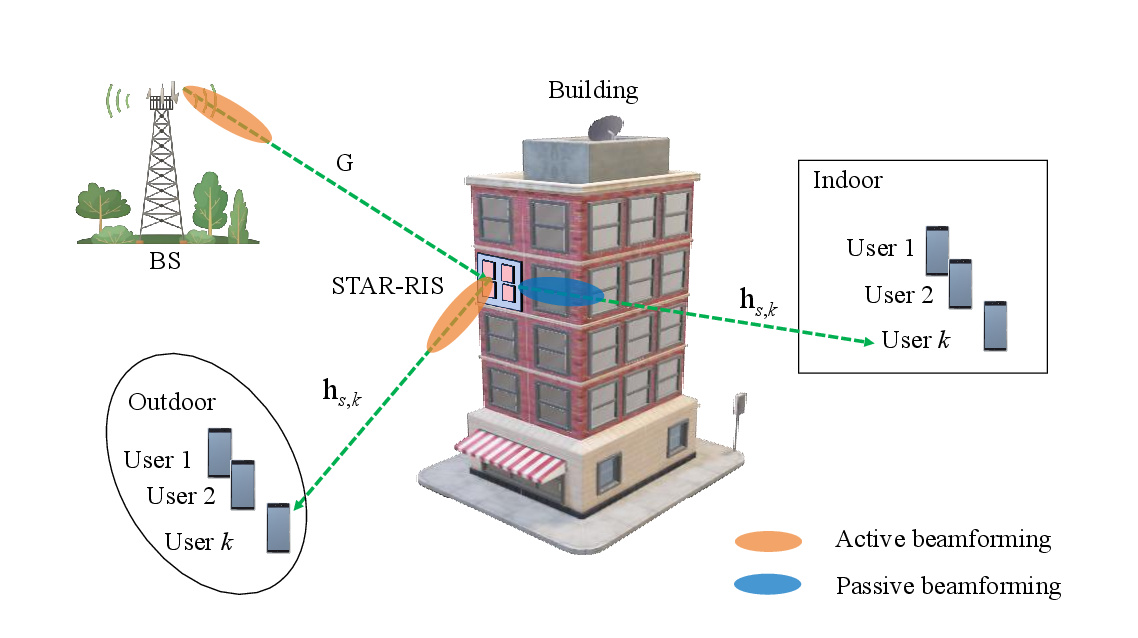
\includegraphics[width=0.90\columnwidth]{systemEE3_clean.jpg}
\caption{Hybrid active-passive STAR-RIS-assisted two-side downlink.}
\label{fig:system}
\end{figure}

Denote by $\mathbf{G}\in\mathbb{C}^{N\times M}$ the BS-to-STAR-RIS channel, and by $\mathbf{h}_{s,k}\in\mathbb{C}^N$ the STAR-RIS-to-user channel on side $s$ for user $k$. The received signal at user $(s,k)$ is
\begin{equation}
y_{s,k}=\mathbf{h}_{s,k}^H\mathbf{\Theta}_s\mathbf{G}
\sum_{q\in\{t,r\}}\sum_{j\in\mathcal{K}_{q}}\mathbf{w}_{q,j}x_{q,j}
+\mathbf{h}_{s,k}^H\mathbf{n}_{a,s}+n_{s,k},
\label{eq:received}
\end{equation}
where $\mathbf{\Theta}_s=\diag(\theta_{1,s},\ldots,\theta_{N,s})$, the summation index $q\in\{t,r\}$ enumerates the side of each transmitted stream, $\mathbf{w}_{q,j}\in\mathbb{C}^{M}$ is the BS beamformer for user $(q,j)$, $x_{q,j}$ is the unit-power information symbol, and $n_{s,k}\sim\mathcal{CN}(0,\sigma_0^2)$ is thermal noise. The vector $\mathbf{n}_{a,s}$ represents the amplified noise contributed by active elements on side $s$. Following the active-RIS noise model in \cite{zhang2022signal,ma2023activeee}, it is modeled as
\begin{equation}
\mathbf{n}_{a,s}\sim\mathcal{CN}(\mathbf{0},\mathbf{C}_{a,s}),\qquad
\mathbf{C}_{a,s}=\diag(c_{1,s},\ldots,c_{N,s}),
\label{eq:na_stat}
\end{equation}
where $c_{n,s}=\rho_{n,s}\beta_{n,s}^2\sigma_a^2$ for $n\in\mathcal{A}_s$ and $c_{n,s}=0$ otherwise, with $\sigma_a^2$ denoting the input-referred active-element noise variance. The SINR of user $(s,k)$ is then
\begin{equation}
\gamma_{s,k}=
\frac{\left|\mathbf{h}_{s,k}^H\mathbf{\Theta}_s\mathbf{G}\mathbf{w}_{s,k}\right|^2}
{\sum_{\substack{q\in\{t,r\},\ j\in\mathcal{K}_{q}\\(q,j)\ne(s,k)}}
\left|\mathbf{h}_{s,k}^H\mathbf{\Theta}_s\mathbf{G}\mathbf{w}_{q,j}\right|^2
+\sigma_{a,s,k}^2+\sigma_0^2},
\label{eq:sinr_full}
\end{equation}
where $\sigma_{a,s,k}^2=\mathbf{h}_{s,k}^H\mathbf{C}_{a,s}\mathbf{h}_{s,k}$ is the active-noise term seen at user $(s,k)$.

\subsection{Power-Consumption Model}
Following measurement-based RIS power models \cite{wang2023static,wang2024practical}, the total consumed power is written as
\begin{equation}
\begin{aligned}
P_{\mathrm{tot}}
&=\frac{1}{\etaPA}
\sum_{s\in\{t,r\}}\sum_{k\in\mathcal{K}_s}\|\mathbf{w}_{s,k}\|^2
+P_{\mathrm{ctrl}}+P_{\mathrm{bias}}|\mathcal{A}|  \\
&\quad +f_u\!\left(E_{\mathrm{sw},0}+E_{\mathrm{sw},1}|\mathcal{A}|\right) \\
&\quad +\sum_{n\in\mathcal{A}_t}\mu_t(\beta_{n,t}^2-1)
+\sum_{n\in\mathcal{A}_r}\mu_r(\beta_{n,r}^2-1),
\end{aligned}
\label{eq:power_model}
\end{equation}
where $\etaPA$ is the BS PA efficiency, $|\mathcal{A}|$ is the number of active elements, $P_{\mathrm{ctrl}}$ is the controller power, $P_{\mathrm{bias}}$ is the per-active-element bias power, $f_u$ is the update frequency, $E_{\mathrm{sw},0}$ and $E_{\mathrm{sw},1}$ are the base and per-active-element switching energies per update, and $\mu_t,\mu_r$ are the gain-dependent amplifier-power coefficients. The four components in \eqref{eq:power_model} are the PA-normalized BS transmit power, static controller/bias power, update-rate-weighted switching power, and gain-dependent amplification power.

\subsection{Equivalent Scalar Model}
To obtain a tractable EE-SE boundary, the full model is reduced to an equivalent scalar form using four standard approximations: residual multiuser leakage in \eqref{eq:sinr_full} is neglected, common side-wise splitting and gain are used with $\rho_{n,s}=\rho_s$ and $\beta_{n,s}=\beta_s$ for $n\in\mathcal{A}_s$, dominant cascaded paths are phase-aligned, and the side target $R_s$ is enforced by assigning the same target $R_s/K_s$ to every user on side $s$, so that the $K_s$ user targets sum to $R_s$.

Let $\mathbf v_{s,k}$ be a normalized post-zero-forcing (post-ZF) BS direction, and let $\mathbf e_n$ be the $n$th canonical basis vector in $\mathbb{R}^N$. The scalar BS-to-element gain is represented by the stream-averaged effective magnitude
\[
|g_n|\triangleq \frac{1}{K_t+K_r}\sum_{q\in\{t,r\}}\sum_{k\in\mathcal{K}_q}\left|\mathbf e_n^T\mathbf{G}\mathbf v_{q,k}\right|.
\]
With $h_{s,k,n}$ denoting the $n$th entry of $\mathbf{h}_{s,k}$, define
\begin{equation}
u_{s,k,n} = |g_n|\,|h_{s,k,n}|.
\label{eq:un}
\end{equation}
The side-wise effective coherent term for user $(s,k)$ is then
\begin{equation}
\psi_{s,k}(\beta_s)=
\sum_{n\in\mathcal{P}_s}\sqrt{\rho_s}u_{s,k,n}
+\beta_s\sum_{n\in\mathcal{A}_s}\sqrt{\rho_s}u_{s,k,n},
\label{eq:psi}
\end{equation}
where $\mathcal{P}_s=\{1,\ldots,N\}\setminus\mathcal{A}_s$ contains passive elements and those active only for the opposite side. The corresponding active-noise term is
\begin{equation}
\zeta_{s,k}(\beta_s)=\sigma_0^2+
\rho_s\beta_s^2\sigma_a^2
\sum_{n\in\mathcal{A}_s}|h_{s,k,n}|^2.
\label{eq:noise_exact}
\end{equation}
Under this equal per-user target, the minimum side power required to meet the side target $R_s$ is
\begin{equation}
p_s^{\min}(\beta_s)=
\sum_{k\in\mathcal{K}_s}
\frac{(2^{R_s/K_s}-1)\zeta_{s,k}(\beta_s)}{\psi_{s,k}^2(\beta_s)}.
\label{eq:minsidepower}
\end{equation}

\section{Problem Formulation}
The sum spectral efficiency is
\begin{equation}
R_\Sigma=\sum_{s\in\{t,r\}}\sum_{k\in\mathcal{K}_s}\log_2(1+\gamma_{s,k}).
\label{eq:sumrate}
\end{equation}
The EE metric $\mathrm{EE}=R_\Sigma/P_{\mathrm{tot}}$ is used throughout. Let $\mathcal X\triangleq\{\mathbf W,\rho_t,\rho_r,\bm\phi,\beta_t,\beta_r,\mathcal A_t,\mathcal A_r\}$. The EE maximization problem is
\begin{equation}
\begin{aligned}
\max_{\mathcal X}
\quad & \frac{R_\Sigma}{P_{\mathrm{tot}}} \\
\text{s.t.}\quad &
\log_2(1+\gamma_{s,k})\ge \bar{R}_{s,k},\ \forall s,k, \\
&
\sum_{s\in\{t,r\}}\sum_{k\in\mathcal{K}_s}\|\mathbf{w}_{s,k}\|^2 \le P_{\max}^{\mathrm{BS}},\\
&
1\le \beta_s\le \beta_{\max},\quad s\in\{t,r\},\\
&
\mathcal{A}_t\cap\mathcal{A}_r=\emptyset,\quad \mathcal{A}=\mathcal{A}_t\cup\mathcal{A}_r,\\
&
\rho_t+\rho_r=1,\quad 0\le \rho_s\le 1,\quad s\in\{t,r\},\\
&
\rho_s\beta_s^2\sigma_a^2 \le \Gamma_s,\quad s\in\{t,r\}.
\end{aligned}
\label{eq:P0}
\end{equation}
Here, $\Gamma_s$ is an optional side-wise noise-injection or hardware-safety limit. Problem \eqref{eq:P0} is non-convex because the fractional objective couples beamforming, STAR-RIS coefficients, side-wise gains, and active-set selection. To trace an achievable EE-SE Pareto tradeoff, the $\epsilon$-constraint scalarization, a standard multicriteria-optimization approach \cite{ehrgott2005multicriteria}, is adopted
\begin{equation}
\begin{aligned}
\mathcal{P}(\epsilon):\quad
\min_{\mathcal X}
\quad & P_{\mathrm{tot}} \\
\text{s.t.}\quad &
R_\Sigma \ge \epsilon, \\
& \text{constraints of \eqref{eq:P0}.}
\end{aligned}
\label{eq:epsilon}
\end{equation}
In the proposed procedure, the generic quality-of-service (QoS) terms are instantiated as $\bar R_{s,k}=R_s/K_s$, with $R_t=\alpha\epsilon$ and $R_r=(1-\alpha)\epsilon$, so that the per-user constraints realize the side targets in \eqref{eq:minsidepower}. Because the procedure uses structured sparse activation and finite grids, the generated curve is an achievable Pareto-frontier approximation rather than a certified global optimum. The model structure is then exploited to derive practical design rules.

\section{Gain Structure}
\subsection{Amplification ON-OFF Criterion}
Given a side-specific active set, the key question is whether the side-wise active gain should be switched on, i.e., whether increasing $\beta_s$ above one improves the side-wise SINR. For convenience, introduce four side-wise worst-case coefficients: $a_s$ is the passive coherent contribution, $b_s$ is the active coherent contribution evaluated at unit gain, $c_s$ is the receiver thermal-noise baseline, and $d_s$ is the active-noise coefficient before multiplication by $\beta_s^2$. They are
\begin{equation}
\begin{aligned}
a_s &= \min_k \sum_{n\in\mathcal{P}_s}\sqrt{\rho_s}u_{s,k,n},\\
b_s &= \min_k \sum_{n\in\mathcal{A}_s}\sqrt{\rho_s}u_{s,k,n},\\
c_s &= \sigma_0^2,\\
d_s &= \max_k \rho_s\sigma_a^2\sum_{n\in\mathcal{A}_s}|h_{s,k,n}|^2 .
\end{aligned}
\label{eq:abcd}
\end{equation}
The minimum in $a_s$ and $b_s$ protects the weakest user in coherent gain, while the maximum in $d_s$ protects the user most exposed to active noise. Substituting $a_s$, $b_s$, $c_s$, and $d_s$ into \eqref{eq:psi} and \eqref{eq:noise_exact}, and dropping the positive per-user power factor $p_{s,k}$ that does not affect monotonicity with respect to $\beta_s$, gives the normalized worst-user SINR lower bound
\begin{equation}
\underline{\gamma}_s(\beta_s)=
\frac{(a_s+b_s\beta_s)^2}{c_s+d_s\beta_s^2}.
\label{eq:surrogate}
\end{equation}
The coherent term grows linearly with $\beta_s$, whereas the injected active noise grows quadratically. Differentiating \eqref{eq:surrogate} gives
\begin{equation}
\frac{\mathrm{d}\underline{\gamma}_s}{\mathrm{d}\beta_s}=
\frac{2(a_s+b_s\beta_s)(b_sc_s-a_sd_s\beta_s)}{(c_s+d_s\beta_s^2)^2}.
\label{eq:surrogate_derivative}
\end{equation}
Thus, at the passive-gain point $\beta_s=1$, amplification is locally useful if
\begin{equation}
\left.\frac{\mathrm{d}\underline{\gamma}_s}{\mathrm{d}\beta_s}\right|_{\beta_s=1}>0
\iff b_sc_s>a_sd_s.
\label{eq:threshold}
\end{equation}
Equation \eqref{eq:threshold} gives the amplification ON-OFF criterion: the active coherent-gain aggregate $b_s$, weighted by the thermal-noise baseline $c_s$, must dominate the passive coherent-gain aggregate $a_s$ weighted by the active-noise coefficient $d_s$. When this inequality holds, amplification is locally beneficial for the SINR lower bound. Otherwise, the corresponding STAR-RIS amplifier should remain inactive during operation. For EE-oriented operation, bias, switching, and amplification-power costs make the ON-OFF decision more restrictive.

\begin{proposition}\label{prop:se_optimal}
For the positive-coefficient hybrid active-passive case with $a_s>0$, $b_s>0$, $c_s>0$, and $d_s>0$, $\underline{\gamma}_s(\beta_s)$ is unimodal on $[1,\beta_{\max}]$. The SE-oriented gain is
\begin{equation}
\beta_{s,\mathrm{SE}}^\star=
\left[\frac{b_sc_s}{a_sd_s}\right]_{[1,\beta_{\max}]},
\label{eq:beta_closed}
\end{equation}
where $[x]_{[l,u]}=\min\{u,\max\{l,x\}\}$. The boundary cases follow from the same derivative behavior. If $b_s=0$, set $\beta_{s,\mathrm{SE}}^\star=1$. If $a_s=0$ with $b_s>0$, or if $d_s=0$ with $b_s>0$, $\underline{\gamma}_s(\beta_s)$ is nondecreasing and $\beta_{s,\mathrm{SE}}^\star=\beta_{\max}$. If $|\mathcal{A}_s|=0$, set $\beta_s=1$.
\end{proposition}

\begin{IEEEproof}
When all four coefficients are positive, the sign of \eqref{eq:surrogate_derivative} is determined only by $b_sc_s-a_sd_s\beta_s$, whose sign changes only once. Hence \eqref{eq:surrogate} is unimodal and the stationary point is $b_sc_s/(a_sd_s)$, clipped to $[1,\beta_{\max}]$. The boundary cases follow directly from \eqref{eq:surrogate_derivative}: $b_s=0$ makes the derivative non-positive, while $a_s=0$ with $b_s>0$ or $d_s=0$ with $b_s>0$ makes \eqref{eq:surrogate} nondecreasing.
\end{IEEEproof}

\subsection{Power-Minimizing Gain}
The gain in \eqref{eq:beta_closed} is SE-oriented because it maximizes the normalized worst-user SINR lower bound and does not include the denominator of EE. In contrast, the $\epsilon$-constraint problem in \eqref{eq:epsilon} minimizes total consumed power at a fixed SE target. Increasing $\beta_s$ may reduce the BS transmit power required by \eqref{eq:minsidepower}, but it also increases active noise and the gain-dependent amplifier power in \eqref{eq:power_model}. Therefore, the SE-oriented gain and the EE-oriented power-minimizing gain generally differ. For a target side rate $R_s$, define the side-wise cost $\Psi_s(\beta_s)$ as the sum of the transmit-power term induced by \eqref{eq:minsidepower} under the worst-user coefficients and the gain-dependent active-amplifier power:
\begin{align}
\Psi_s(\beta_s)
&=\frac{K_s(2^{R_s/K_s}-1)(c_s+d_s\beta_s^2)}{\etaPA(a_s+b_s\beta_s)^2}
+\mu_s|\mathcal{A}_s|(\beta_s^2-1),
\label{eq:side_cost}\\
\Psi_s'(\beta_s)
&=\frac{2K_s(2^{R_s/K_s}-1)(a_sd_s\beta_s-b_sc_s)}{\etaPA(a_s+b_s\beta_s)^3}
+2\mu_s|\mathcal{A}_s|\beta_s,
\label{eq:side_derivative}\\
\Psi_s''(\beta_s)
&=\frac{2K_s(2^{R_s/K_s}-1)}{\etaPA(a_s+b_s\beta_s)^4}
\Big(a_s^2d_s-2a_sb_sd_s\beta_s+3b_s^2c_s\Big) \notag\\
&\quad +2\mu_s|\mathcal{A}_s|.
\label{eq:side_second}
\end{align}

\begin{proposition}\label{prop:convexity}
Assume the hybrid active-passive case $a_s>0$, $b_s>0$, and $d_s>0$. Under the condition
\begin{equation}
\beta_{\max}
\le
\frac{a_s^2d_s+3b_s^2c_s}{2a_sb_sd_s},
\label{eq:convexity_cond}
\end{equation}
$\Psi_s(\beta_s)$ is strictly convex on $[1,\beta_{\max}]$. Consequently, the side-wise power-minimizing gain is unique and can be obtained by checking the two endpoints and the interior stationary point solving \eqref{eq:side_derivative}, if that point lies in $[1,\beta_{\max}]$.
\end{proposition}

\begin{IEEEproof}
Under \eqref{eq:convexity_cond}, the bracketed term in \eqref{eq:side_second} is non-negative on $[1,\beta_{\max}]$. Since $|\mathcal{A}_s|>0$ and $\mu_s>0$, the term $2\mu_s|\mathcal{A}_s|$ yields $\Psi_s''(\beta_s)>0$ over the interval. Hence $\Psi_s$ is strictly convex and has a unique minimizer.
\end{IEEEproof}


Condition \eqref{eq:convexity_cond} is sufficient but not necessary. When it is violated, $\Psi_s(\beta_s)$ can still be minimized efficiently on the bounded interval $[1,\beta_{\max}]$ by a one-dimensional line search. If no active element is assigned to side $s$, or if the selected elements produce no active coherent term ($b_s=0$), the gain is set to $\beta_s=1$ because increasing it cannot reduce the required power.



\section{Sparse Active Selection and Gain Control}
For a target sum-SE level $\epsilon$ in \eqref{eq:epsilon}, this section constructs one feasible candidate of $\mathcal P(\epsilon)$. The target is split into side rates by $R_t=\alpha\epsilon$ and $R_r=(1-\alpha)\epsilon$, where $\alpha\in\mathcal G_\alpha$, while $L\in\mathcal L$ specifies the number of active elements. Use $x_{n,s}\in\{0,1\}$, $s\in\{t,r\}$, with $x_{n,s}=1$ iff element $n$ is active on side $s$. The constraints $x_{n,t}+x_{n,r}\le 1$ and $\sum_{n=1}^{N}(x_{n,t}+x_{n,r})=L$ impose side-exclusive activation with $L$ active elements; $x_{n,t}=x_{n,r}=0$ denotes a passive element, and $\mathcal A_s=\{n:x_{n,s}=1\}$. Rather than solve the exact combinatorial program, Algorithm~\ref{alg:selection_gain} constructs ranked binary candidates and evaluates them under the scalar model.

\subsection{Step 1: Selecting \texorpdfstring{$L$}{L} Active Elements}
For fixed $(L,\alpha)$, an element is useful if its coherent-gain contribution can reduce the BS power more than its added active-noise and hardware-power costs. Let
\[
C_s=\frac{K_s(2^{R_s/K_s}-1)}{\etaPA},
\]
which collects the side-rate and PA-efficiency factors in the transmit-power term of \eqref{eq:side_cost}. To derive a ranking score, introduce a temporary continuous insertion variable $\chi_{n,s}\in[0,1]$ only for local sensitivity analysis. The final decision variable remains the binary $x_{n,s}$ defined above.

If element $n$ is tentatively inserted on side $s$, its worst-user coherent increment is $\Delta u_{n,s}=\sqrt{\rho_s}|g_n|\min_k|h_{s,k,n}|$, and its active-noise increment is approximated by $\Delta d_{n,s}\approx\rho_s\sigma_a^2\mathbb E_k[|h_{s,k,n}|^2]$, where $\mathbb E_k[\cdot]\triangleq K_s^{-1}\sum_{k\in\mathcal K_s}(\cdot)$ is the empirical user average on side $s$. With $D_{n,s}(\chi_{n,s})=a_s+b_s\beta_s+(\beta_s-1)\chi_{n,s}\Delta u_{n,s}$, the insertion-relaxed side cost is approximated as
\[
\begin{aligned}
\Psi_s(\chi_{n,s})
&\approx C_s\big[c_s+\beta_s^2(d_s+\chi_{n,s}\Delta d_{n,s})\big]
D_{n,s}^{-2}(\chi_{n,s}) \\
&\quad +\mu_s(|\mathcal A_s|+\chi_{n,s})(\beta_s^2-1) \\
&\quad +\chi_{n,s}(P_{\mathrm{bias}}+f_uE_{\mathrm{sw},1}).
\end{aligned}
\]
Differentiating at $\chi_{n,s}=0$ gives the first-order benefit ratio
\[
\tilde{\xi}_{n,s}\triangleq
\frac{\kappa_{1,s}\Delta u_{n,s}}
{\kappa_{2,s}\Delta d_{n,s}+P_{\mathrm{bias}}+f_uE_{\mathrm{sw},1}+\mu_s(\beta_s^2-1)},
\]
where
\[
\begin{aligned}
\kappa_{1,s}&=\frac{2C_s(c_s+d_s\beta_s^2)(\beta_s-1)}{(a_s+b_s\beta_s)^3},\\
\kappa_{2,s}&=\frac{C_s\beta_s^2}{(a_s+b_s\beta_s)^2}.
\end{aligned}
\]
A value $\tilde{\xi}_{n,s}>1$ indicates that the first-order coherent-gain saving dominates the active-noise, bias, switching, and amplifier-power penalties. For a non-iterative implementation, use side weights $\omega_t=\alpha$ and $\omega_r=1-\alpha$ and define the normalized score
\begingroup\small
\begin{equation}
\xi_{n,s}=\frac{\omega_s\Delta u_{n,s}}
{\sigma_0^{-2}\Delta d_{n,s}+(P_{\max}^{\mathrm{BS}})^{-1}(P_{\mathrm{bias}}+f_uE_{\mathrm{sw},1})},\quad s\in\{t,r\}.
\label{eq:score}
\end{equation}
\endgroup
The numerator is the side-weighted coherent increment, while the denominator normalizes the active-noise increment and per-active-element hardware overhead.

\subsection{Step 2: Assigning Active Elements to Sides}
For each $(L,\alpha)$, two candidate active-set pairs are constructed by the same rule: choose each element's preferred side, retain the $L$ largest preferred scores, and split the retained indices according to their preferred sides. For the cost-aware pair, define $s_n^{\mathrm{ca}}=\arg\max_{s\in\{t,r\}}\xi_{n,s}$ and $\xi_n^{\mathrm{ca}}=\xi_{n,s_n^{\mathrm{ca}}}$. Let $\mathcal S^{\mathrm{ca}}$ contain the $L$ largest values of $\xi_n^{\mathrm{ca}}$, and set $\mathcal A_s^{\mathrm{ca}}=\{n\in\mathcal S^{\mathrm{ca}}:s_n^{\mathrm{ca}}=s\}$ for $s\in\{t,r\}$. Thus, selection and side assignment are coupled by the same score.

The second pair is channel-strength based and is used as the strongest-greedy baseline in Sec.~VI. It removes the denominator of \eqref{eq:score} and uses $\pi_{n,s}=\omega_s\Delta u_{n,s}$. With $s_n^{\mathrm{st}}=\arg\max_{s\in\{t,r\}}\pi_{n,s}$ and $\pi_n^{\mathrm{st}}=\pi_{n,s_n^{\mathrm{st}}}$, the $L$ largest values of $\pi_n^{\mathrm{st}}$ form $\mathcal S^{\mathrm{st}}$, and $\mathcal A_s^{\mathrm{st}}=\{n\in\mathcal S^{\mathrm{st}}:s_n^{\mathrm{st}}=s\}$ for $s\in\{t,r\}$. Both candidate pairs are evaluated in Algorithm~\ref{alg:selection_gain}.

\subsection{Step 3: Updating \texorpdfstring{$(\beta_t,\beta_r)$}{(beta t, beta r)}}
For each candidate pair $(\mathcal A_t,\mathcal A_r)$, the coefficients $(a_s,b_s,c_s,d_s)$ are computed from \eqref{eq:abcd}. The boundary cases in Proposition~\ref{prop:se_optimal} are handled by setting $\beta_s=1$ when $|\mathcal A_s|=0$ or $b_s=0$. Otherwise, the EE-oriented gain is updated by
\[
\beta_s^\star=\arg\min_{1\le\beta_s\le\beta_{\max}}\Psi_s(\beta_s),
\]
where $\Psi_s(\beta_s)$ is given in \eqref{eq:side_cost}. The updated gains determine the required side powers $p_t^{\min}(\beta_t^\star)$ and $p_r^{\min}(\beta_r^\star)$ through \eqref{eq:minsidepower}.

\subsection{Step 4: Feasibility Check and Boundary-Point Selection}
After the gain update, each candidate is checked against the scalar-model version of \eqref{eq:P0}: the BS transmit-power budget, the gain bounds, the non-overlapping active-set constraint, the ES splitting constraints, and the optional safety cap $\Gamma_s$. Among all feasible candidates for the current target $\epsilon$, the returned boundary point is
\[
\mathcal B^\star=\big(\mathcal A_t^\star,\mathcal A_r^\star,\beta_t^\star,\beta_r^\star,
\alpha^\star,p_t^{\min,\star},p_r^{\min,\star},P_{\mathrm{tot}}^\star,
\mathrm{EE}^\star\big),
\]
where $P_{\mathrm{tot}}^\star$ is the smallest feasible value of \eqref{eq:power_model} and $\mathrm{EE}^\star=\epsilon/P_{\mathrm{tot}}^\star$. The complete procedure is summarized in Algorithm~\ref{alg:selection_gain}.

\begin{algorithm}[H]
\caption{Sparse Active Selection and Gain Control}
\label{alg:selection_gain}
\footnotesize
\begin{algorithmic}[1]
\State \textbf{Initialize:} $P_{\min}=+\infty$ and $\mathcal B^\star=\emptyset$.
\ForAll{$(L,\alpha)\in\mathcal L\times\mathcal G_\alpha$}
    \State $R_t=\alpha\epsilon$ and $R_r=(1-\alpha)\epsilon$.
    \State Form $(\mathcal A_t^{\mathrm{ca}},\mathcal A_r^{\mathrm{ca}})$ using $\xi_{n,s}$ in \eqref{eq:score}.
    \State Form $(\mathcal A_t^{\mathrm{st}},\mathcal A_r^{\mathrm{st}})$ using $\pi_{n,s}$.
    \ForAll{$(\mathcal A_t,\mathcal A_r)\in\{(\mathcal A_t^{\mathrm{ca}},\mathcal A_r^{\mathrm{ca}}),(\mathcal A_t^{\mathrm{st}},\mathcal A_r^{\mathrm{st}})\}$}
        \State Compute $(a_s,b_s,c_s,d_s)$ from \eqref{eq:abcd} for $s\in\{t,r\}$.
        \State For each $s$, \textbf{if} $|\mathcal A_s|=0$ or $b_s=0$, set $\beta_s^\star=1$.
        \State \textbf{Otherwise}
        \Statex \hspace{\algorithmicindent} set $\beta_s^\star=\arg\min_{1\le\beta_s\le\beta_{\max}}\Psi_s(\beta_s)$ for that side.
        \State Compute $p_t^{\min}$, $p_r^{\min}$, and $P_{\mathrm{tot}}$ from \eqref{eq:minsidepower} and \eqref{eq:power_model}.
        \State \textbf{If} constraints of \eqref{eq:P0} hold and $P_{\mathrm{tot}}<P_{\min}$, set $P_{\min}=P_{\mathrm{tot}}$
        \Statex \hspace{\algorithmicindent} and $\mathcal B^\star=(\mathcal A_t,\mathcal A_r,\beta_t^\star,\beta_r^\star,\alpha,p_t^{\min},p_r^{\min},P_{\mathrm{tot}},\epsilon/P_{\mathrm{tot}})$.
    \EndFor
\EndFor
\State \textbf{If} $\mathcal B^\star=\emptyset$, \textbf{return} $\emptyset$.
\State \textbf{Otherwise} \textbf{return} $\mathcal B^\star$.
\end{algorithmic}
\vspace{-0.5ex}
\end{algorithm}

\subsection{Complexity}
Let $G=|\mathcal{G}_{\alpha}|$, $L_g=|\mathcal{L}|$, $K=K_t+K_r$, and $Q_\beta$ denote the bounded one-dimensional gain-search budget. For each boundary point, score computation, sorting, active-set evaluation, and gain update require $\mathcal{O}(L_gG(N\log N+NK+Q_{\beta}))$ operations. For $E$ sampled SE targets, the total complexity is $\mathcal{O}(E L_gG(N\log N+NK+Q_{\beta}))$, and the memory cost is dominated by channel coefficients and element scores.


\section{Numerical Results}
In this section, simulations evaluate the achievable EE-SE boundary, hardware sensitivity, and power distribution of the proposed sparse active-selection design. Unless otherwise stated, the STAR-RIS has $N=24$ elements and serves $K_t=K_r=2$ users. The channels follow Nakagami-$m$ fading with $\mBR=\mRU=1$ and normalized average link-power scalings $\Omega_{BR}=0.20$, $\Omega_t=(0.060,0.050)$, and $\Omega_r=(0.080,0.060)$. We use $(\rho_t,\rho_r)=(0.55,0.45)$, $\beta_{\max}=5$, $P_{\max}^{\mathrm{BS}}=5$ W, $\sigma_0^2=6.25\times10^{-2}$, $\sigma_a^2=2.5\times10^{-3}$, and $\etaPA=0.40$. The search grids are $\mathcal G_\alpha=\{0.20,0.25,\ldots,0.80\}$ and $\mathcal L=\{0,3,\ldots,24\}$. Hardware-power coefficients follow measured RIS power models and are set to $P_{\mathrm{ctrl}}=0.10$ W, $P_{\mathrm{bias}}=0.015$ W, $f_u=50$ Hz, $(E_{\mathrm{sw},0},E_{\mathrm{sw},1})=(2.0,1.2)\times10^{-4}$ J, and $\mu_t=\mu_r=2.5\times10^{-3}$ W \cite{wang2023static,wang2024practical}. These settings follow common two-side STAR-RIS layouts \cite{mu2022star}, hybrid/active RIS EE studies and active-noise models \cite{ma2023activeee,peng2023hybrid,zhang2022signal,zhang2023activevspassive}, and Nakagami-$m$ RIS channel analysis \cite{ni2023nakagami}. Each plotted Monte Carlo (MC) point averages independent channel realizations generated by the reproducibility script.

The baselines include passive ($L=0$), active ($L=N$), fixed/optimized uniform, single-random sparse, strongest greedy, reweighted-$\ell_1$ sparse selection \cite{long2024poweraware}, and hybrid AO/SCA refinement \cite{nguyen2022hybrid}.

Fig.~\ref{fig:pareto} shows the EE-SE boundary and the main power-allocation tradeoff. Passive STAR-RIS is competitive at low SE, but its BS-power requirement grows rapidly with $R_\Sigma$ and becomes infeasible when it exceeds $P_{\max}^{\mathrm{BS}}$. The unfilled passive markers at high $R_\Sigma$ are averaged over feasible trials only. The active benchmark lowers BS power but incurs substantial static, switching, and amplification overhead. The proposed, strongest-greedy, reweighted-$\ell_1$, and AO/SCA-refined curves are close in this setup because their selected active sets often overlap, while the proposed ranker keeps the finite-grid search cost-aware by penalizing active noise and hardware costs.

\begin{figure}[H]
\centering
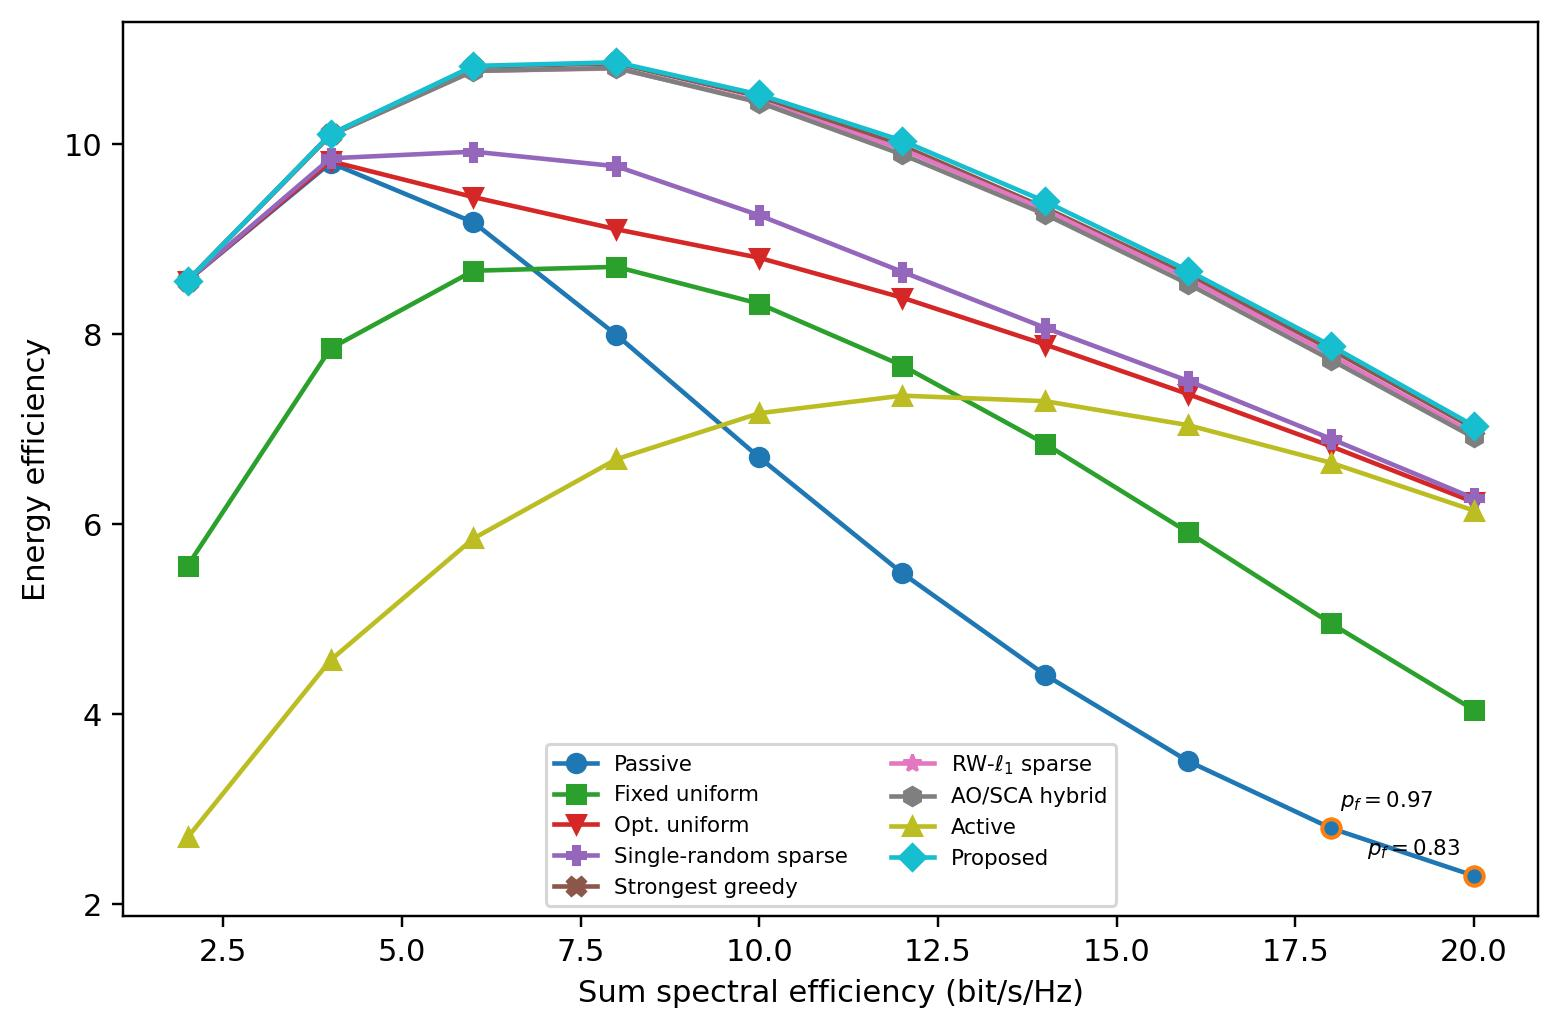
\includegraphics[width=0.80\columnwidth]{fig_pareto_boundary.jpg}
\caption{Approximated EE-SE boundary.}
\label{fig:pareto}
\end{figure}


Fig.~\ref{fig:noise_dyn} shows hardware sensitivity at $R_\Sigma=6$, $9$, $12$, $15$, and $18$ bit/s/Hz. A larger gain is not always beneficial: increasing $\sigma_a$ suppresses the selected gain because amplifier noise scales with $\beta_s^2$ and raises the required power. Increasing $f_u$ similarly increases switching power and reduces EE.

\begin{figure}[H]
\centering
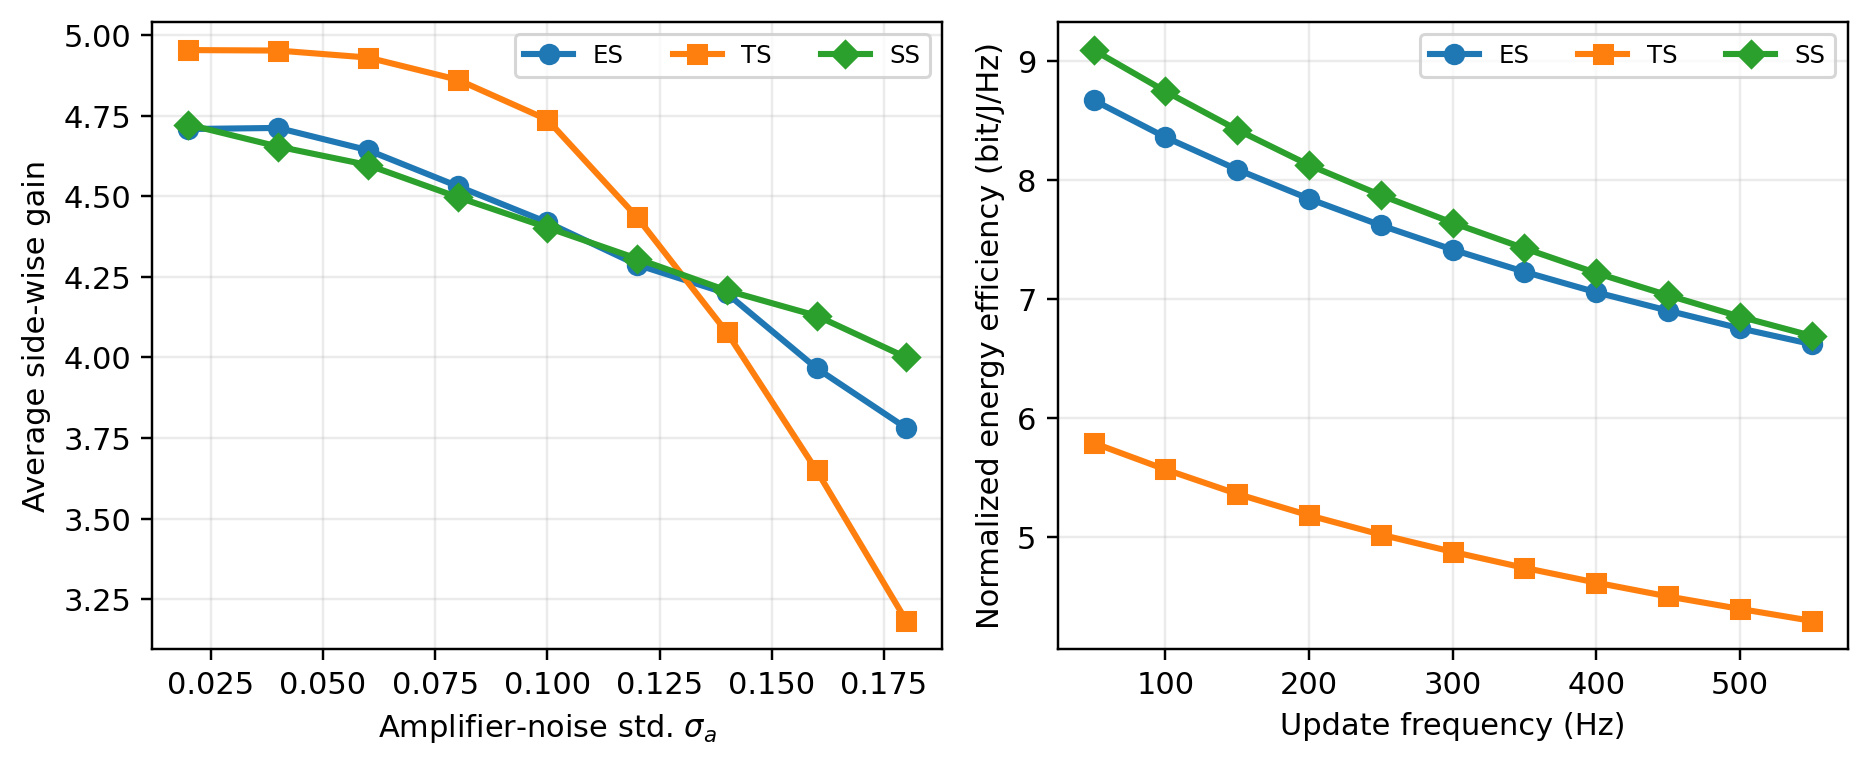
\includegraphics[width=0.90\columnwidth]{fig_noise_dynamic.jpg}
\caption{Hardware sensitivity versus amplifier noise and switching overhead.}
\label{fig:noise_dyn}
\end{figure}

Fig.~\ref{fig:breakdown} compares the power distribution at $R_\Sigma=12$ and $16$ bit/s/Hz. The bars are sorted by total consumed power in descending order. Active operation reduces the BS transmit-power component but incurs large static, switching, and amplification overhead. Sparse active designs balance these terms, which explains why activating only a subset of elements is preferable to either fully passive or fully active operation.

\begin{figure}[H]
\centering
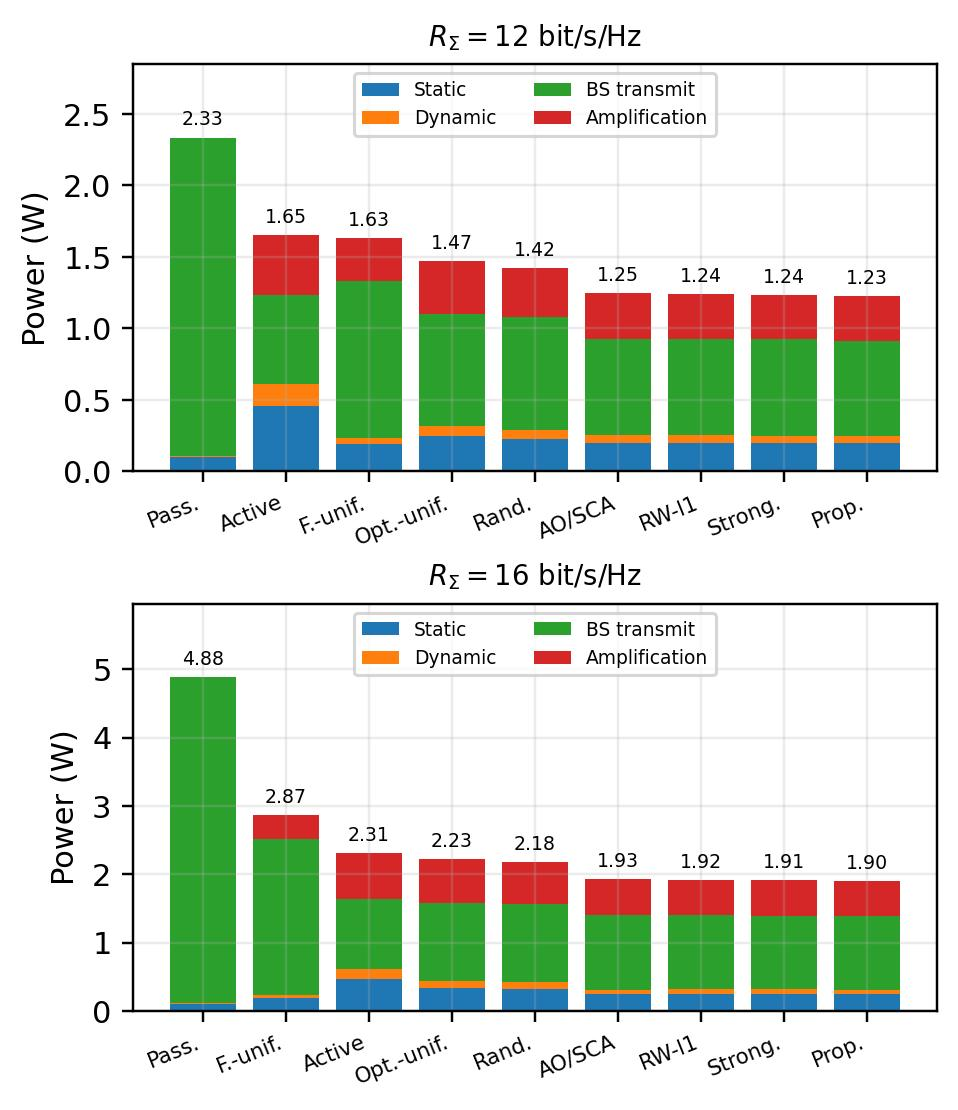
\includegraphics[width=0.96\columnwidth]{fig_power_breakdown.jpg}
\caption{Power distribution at $R_\Sigma=12$ and $16$ bit/s/Hz, sorted by total power.}
\label{fig:breakdown}
\end{figure}

Fig.~\ref{fig:runtime_n} reports the measured runtime per boundary point as the number of STAR-RIS elements increases. The timing test is separate from MC averaging and uses the same finite-grid search structure as the boundary-generation procedure. The proposed method evaluates both cost-aware and channel-strength candidate pairs, so its runtime is higher than a single-ranker baseline but remains governed by the finite grid.

\begin{figure}[H]
\centering
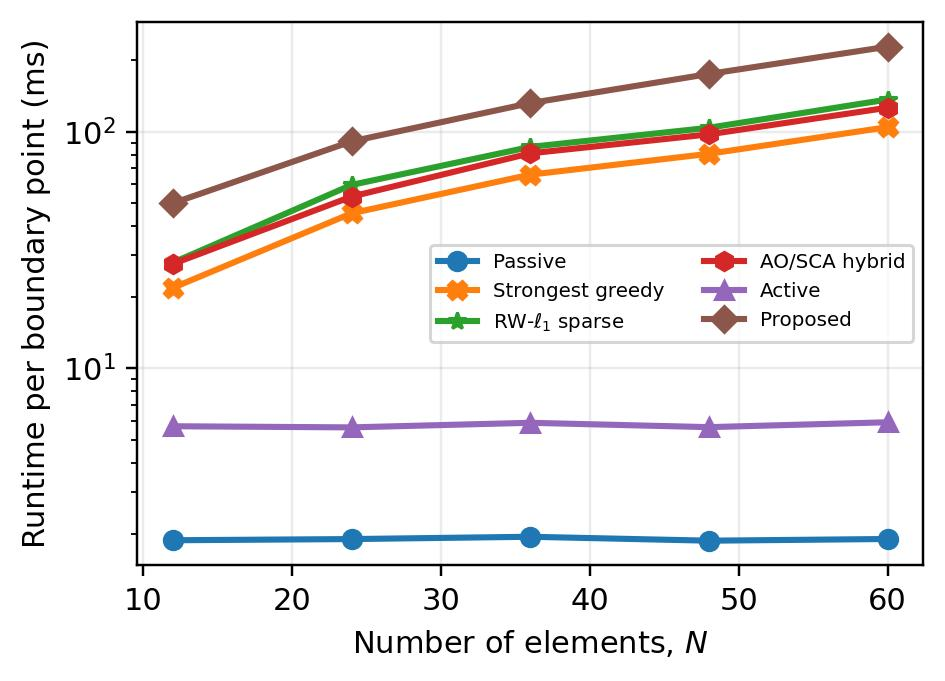
\includegraphics[width=0.82\columnwidth]{fig_runtime_vs_N.jpg}
\caption{Runtime per boundary point versus the number of STAR-RIS elements.}
\label{fig:runtime_n}
\end{figure}

Fig.~\ref{fig:ee_runtime} shows the EE-runtime tradeoff at $R_\Sigma=12$ bit/s/Hz. The proposed design provides the largest EE among the compared scalar-model schemes in this setting, while the passive and fully active designs have lower computational cost but lower EE.

\begin{figure}[H]
\centering
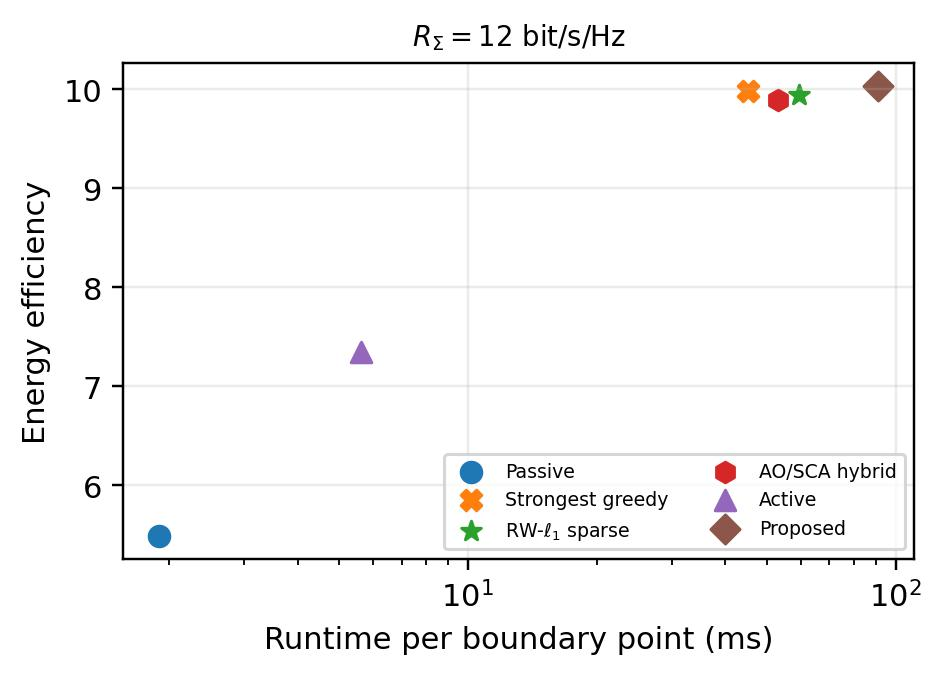
\includegraphics[width=0.82\columnwidth]{fig_ee_runtime_tradeoff.jpg}
\caption{EE-runtime tradeoff at $R_\Sigma=12$ bit/s/Hz.}
\label{fig:ee_runtime}
\end{figure}

\section{Conclusion}
This letter studied the EE-SE behavior of hybrid active-passive STAR-RIS under sparse active selection and gain control. The numerical results indicate that the best EE is obtained at a moderate active density: too few active elements leave a large BS transmit-power demand, whereas too many elements amplify noise and accumulate hardware power. The cost-aware selection improves the achievable EE-SE boundary by avoiding elements whose coherent-channel gain is outweighed by active-noise and hardware penalties. Since the procedure uses structured sparse activation and finite grids, the resulting curve is an achievable Pareto-frontier approximation with practical design value, rather than a certified globally optimal Pareto frontier. The power distribution further confirms that switching, bias, and gain-dependent amplifier terms are decisive in determining when active STAR-RIS operation is energy efficient. Future work will validate the design under full-dimensional beamforming and incorporate signal-dependent active-output constraints.

\begingroup
\renewcommand{\baselinestretch}{0.70}\selectfont
\fontsize{5.2}{5.2}\selectfont

\begin{thebibliography}{99}
\setlength{\itemsep}{0pt}
\setlength{\parskip}{0pt}

\bibitem{wu2019irs}
Q.~Wu and R.~Zhang,
``Intelligent reflecting surface enhanced wireless network via joint active and passive beamforming,''
\emph{IEEE Trans. Wireless Commun.}, vol.~18, no.~11, pp.~5394--5409, Nov.~2019.

\bibitem{bjornson2020irsrelay}
E.~Bj{\"o}rnson, {\"O}.~{\"O}zdogan, and E.~G. Larsson,
``Intelligent reflecting surface versus decode-and-forward: How large surfaces are needed to beat relaying?,''
\emph{IEEE Wireless Commun. Lett.}, vol.~9, no.~2, pp.~244--248, Feb.~2020.

\bibitem{bjornson2020myths}
E.~Bj{\"o}rnson, {\"O}.~{\"O}zdogan, and E.~G. Larsson,
``Reconfigurable intelligent surfaces: Three myths and two critical questions,''
\emph{IEEE Commun. Mag.}, vol.~58, no.~12, pp.~90--96, Dec.~2020.

\bibitem{liu2021star}
Y.~Liu, X.~Mu, J.~Xu, R.~Schober, Y.~Hao, H.~V. Poor, and L.~Hanzo,
``STAR: Simultaneous transmission and reflection for 360$^\circ$ coverage by intelligent surfaces,''
\emph{IEEE Wireless Commun.}, vol.~28, no.~6, pp.~102--109, Dec.~2021.

\bibitem{mu2022star}
X.~Mu, Y.~Liu, L.~Guo, J.~Lin, and R.~Schober,
``Simultaneously transmitting and reflecting (STAR) RIS aided wireless communications,''
\emph{IEEE Trans. Wireless Commun.}, vol.~21, no.~5, pp.~3083--3098, May~2022.

\bibitem{xu2023activestar}
J.~Xu, J.~Zuo, J.~T. Zhou, and Y.~Liu,
``Active simultaneously transmitting and reflecting (STAR)-RISs: Modelling and analysis,''
\emph{IEEE Commun. Lett.}, vol.~27, no.~9, pp.~2466--2470, Sep.~2023.

\bibitem{ma2023activeee}
Y.~Ma, M.~Li, Y.~Liu, Q.~Wu, and Q.~Liu,
``Active reconfigurable intelligent surface for energy efficiency in MU-MISO systems,''
\emph{IEEE Trans. Veh. Technol.}, vol.~72, no.~3, pp.~4103--4107, Mar.~2023.

\bibitem{peng2023hybrid}
Q.~Peng, Q.~Wu, G.~Chen, R.~Liu, S.~Ma, and W.~Chen,
``Hybrid active-passive IRS assisted energy-efficient wireless communication,''
\emph{IEEE Commun. Lett.}, vol.~27, no.~8, pp.~2202--2206, Aug.~2023.

\bibitem{huang2024hybrid}
A.~Huang, X.~Mu, L.~Guo, and G.~Zhu,
``Hybrid active-passive RIS transmitter enabled energy-efficient multi-user communications,''
\emph{IEEE Trans. Wireless Commun.}, vol.~23, no.~9, pp.~10653--10666, Sep.~2024.

\bibitem{nguyen2022hybrid}
N.~T. Nguyen, V.-D. Nguyen, Q.~Wu, A.~T{\"o}lli, S.~Chatzinotas, and M.~Juntti,
``Hybrid active-passive reconfigurable intelligent surface-assisted multi-user MISO systems,''
in \emph{Proc. IEEE SPAWC}, Oulu, Finland, 2022, pp.~1--5.

\bibitem{long2024poweraware}
R.~Long, H.~Zhou, and Y.-C. Liang,
``Power-aware sparse reflect beamforming in active RIS-aided interference channels,''
\emph{IEEE Internet Things J.}, vol.~11, no.~22, pp.~37057--37070, Nov.~2024.


\bibitem{zhang2022signal}
Z.~Zhang, L.~Dai, X.~Chen, C.~Liu, F.~Yang, R.~Schober, and H.~V. Poor,
``Active RISs: Signal modeling, asymptotic analysis, and beamforming design,''
in \emph{Proc. IEEE GLOBECOM}, Rio de Janeiro, Brazil, 2022, pp.~1618--1624.

\bibitem{zhang2023activevspassive}
Z.~Zhang, L.~Dai, X.~Chen, C.~Liu, F.~Yang, R.~Schober, and H.~V. Poor,
``Active RIS vs. passive RIS: Which will prevail in 6G?,''
\emph{IEEE Trans. Commun.}, vol.~71, no.~3, pp.~1707--1725, Mar.~2023.

\bibitem{ni2023nakagami}
Y.~Ni, H.~Zhao, Y.~Liu, J.~Wang, G.~Gui, and H.~Zhang,
``Analysis of RIS-aided communications over Nakagami-$m$ fading channels,''
\emph{IEEE Trans. Veh. Technol.}, vol.~72, no.~7, pp.~8709--8721, Jul.~2023.

\bibitem{wang2023static}
J.~Wang, W.~Tang, S.~Jin, X.~Li, and M.~Matthaiou,
``Static power consumption modeling and measurement of reconfigurable intelligent surfaces,''
in \emph{Proc. EUSIPCO}, Helsinki, Finland, 2023, pp.~890--894.

\bibitem{wang2024practical}
J.~Wang, W.~Tang, J.~C. Liang, L.~Zhang, J.~Y. Dai, X.~Li, S.~Jin, Q.~Cheng, and T.~J. Cui,
``Reconfigurable intelligent surface: Power consumption modeling and practical measurement validation,''
\emph{IEEE Trans. Commun.}, vol.~72, no.~9, pp.~5720--5734, Sep.~2024.

\bibitem{ehrgott2005multicriteria}
M.~Ehrgott,
\emph{Multicriteria Optimization}, 2nd~ed.
Berlin, Germany: Springer, 2005.

\end{thebibliography}
\endgroup

\end{document}
